This chapter explains how the portfolio problem can be treated as a
Markov Decision Process (MDP)~\cite{bellman1957, sutton2018}, i.e the trading process is treated as a
sequence of step-by-step decision-making problems. The objective is to
develop an environment in which an autonomous trading agent can learn an
optimal decision-making behaviour by interacting with a simulated
market. At each step, the portfolio system observes current market and
portfolio conditions, takes an action such as buying, selling, or
holding, receives a result based on how the portfolio's wealth changed,
and then moves to the next step.

The chapter then explains the two main learning methods used in the
project: \textbf{REINFORCE}~\cite{williams1992}---the Monte-Carlo policy gradient, which
learns by improving its strategy based on the rewards it receives ---and
\textbf{Deep Q-learning}~\cite{watkins1992, mnih2015}, which learns which actions are likely to give
the best results. Finally, \textbf{PPO} is introduced as an additional
method in the ablation row to compare against the other approaches, as
it is designed to make the policy learning process more stable.

Table 3.1 collects every symbol used for reference.

\addcontentsline{lot}{table}{\protect\numberline{3.1}{Notation used throughout Chapters 3--5.}}
\textbf{Table 3.1: Notation used throughout Chapters 3--5.}

{\def\LTcaptype{none} % do not increment counter
\begin{longtable}[]{@{}
  >{\raggedright\arraybackslash}p{(\linewidth - 2\tabcolsep) * \real{0.1885}}
  >{\raggedright\arraybackslash}p{(\linewidth - 2\tabcolsep) * \real{0.8115}}@{}}
\toprule\noalign{}
\begin{minipage}[b]{\linewidth}\raggedright
\textbf{Symbol}
\end{minipage} & \begin{minipage}[b]{\linewidth}\raggedright
\textbf{Meaning}
\end{minipage} \\
\midrule\noalign{}
\endhead
\bottomrule\noalign{}
\endlastfoot
\emph{s\textsubscript{t}} ∈ ℝ\textsuperscript{9} & state observed by the
agent at trading day t, containing the nine features used by the
trading system (Table 3.3) \\
\rowsep
\emph{a\textsubscript{t}} ∈ \{0, 1, 2\} & action selected by the agent:
Hold, Buy, or Sell. \\
\rowsep
\emph{P\textsubscript{t}} & asset price at day trading t; \\
\rowsep
\emph{r\textsubscript{t}} & reward received after an action, calculated
from the change in portfolio value after transaction costs. \\
\rowsep
\emph{C\textsubscript{t}} & amount of cash available to the agent at
trading day t \\
\rowsep
\emph{h\textsubscript{t}} & number of (fractional) units of the asset
held at trading day t. \\
\rowsep
\emph{W\textsubscript{t}} = \emph{C\textsubscript{t}} +
\emph{h\textsubscript{t}} \emph{P\textsubscript{t}} & Total portfolio
value, calculated as untouched cash plus the current value of the asset
held; \\
\rowsep
\emph{C\textsubscript{0}} & initial cash available at the beginning of
an episode. \\
\rowsep
\emph{c} & proportional transaction fee for taking a trade, set to
0.05\% per transaction \\
\rowsep
\emph{Δ} = \emph{f} \emph{C\textsubscript{0}} & fixed monetary size of
each trade; the fraction \emph{f} is selected on validation data
(Section 5.3) \\
\rowsep
\emph{γ} & discount factor used to determine the importance of future
rewards \\
\rowsep
\emph{τ} & a trajectory (one complete trading episode), corresponding to
one month of daily trading; related to \emph{t \& T} \\
\rowsep
\emph{T} & episode length in days (with 𝑇 ≈18--23) \\
\rowsep
\emph{t} & 1 trading day \\
\rowsep
\emph{G}(τ) & The total return obtained over a complete episode \\
\rowsep
\emph{G\textsubscript{t}} & The accumulated future reward from time t
onwards. \\
\rowsep
\emph{π\textsubscript{θ}}(\emph{a} \textbar{} \emph{s}) & policy network
that determines the likelihood of choosing action \emph{a} given the
current state \emph{s}. \\
\rowsep
\emph{Q\textsubscript{φ}}(s, \emph{a}) & The Q-network, which estimates
the value of taking a particular action in a given state; frozen target
copy \\
\rowsep
\emph{Q\textsubscript{φ⁻}} & A fixed copy of the Q-network used as a
target during Deep Q-learning. \\
\rowsep
\emph{J}(θ) & objective function representing the expected return of the
policy \\
\rowsep
\emph{ε} & exploration rate used by the (ε-greedy) action-selection
strategy \\
\end{longtable}
}

\section{Overview: Trading as a Markov Decision Process}

Reinforcement Learning (RL) trains an agent to make sequential decisions
by interacting with an environment. The environment is modelled as an
MDP where decisions are made at regular time steps, represented by the
tuple~\(\left( \mathcal{S},\mathcal{A},\mathcal{P},\mathcal{R},\gamma \right)\):
at step \(t\) the agent observes the current state \(s_{t} \in S\),
selects an action \(a_{t} \in A\), receives a numerical reward based on
the outcome \(r_{t}\), and the environment moves to the next state
\(s_{t + 1}\) according to the current state and the action selected by
the agent \(P(s_{t + 1}|s_{t},a_{t})\).

In this project, the trading environment is modelled in the same way,
providing a formal description of how the trading agent interacts with
the market over time; one time step \(t\) corresponds to one trading
day.

The state \(s_{t}\) represents all information available to the agent on
day \(t\) to fully capture its position within the trading episode. This
includes the selected market features, the agent\textquotesingle s
current portfolio position, and its available cash.

Based on this state, the agent selects one of three possible actions
\(a_{t} \in \left\{ 0,\ 1,\ 2 \right\}\): \emph{Hold the current
position, Buy a fixed amount, or Sell a fixed amount.} The selected
trade is then executed, with transaction fees \(c\) applied where
appropriate.

After taking an action, the environment calculates the change in the
agent\textquotesingle s total portfolio value and returns it as the
reward \(r_{t}\).

The environment advances to the next trading day \(s_{t + 1}\), and the
process repeats throughout the episode \emph{τ}, allowing the agent to
update its policy \(\pi_{\theta}\) or value estimates \(Q_{\phi}\) based
on the experience collected.

The interaction can therefore be represented as:
\(s_{t} \rightarrow a_{t} \rightarrow r_{t},s_{t + 1}\)

\textbf{Figure 3.1 illustrates the interaction between the trading agent
and the environment.}

\begin{figure}[!htb]
  \centering
  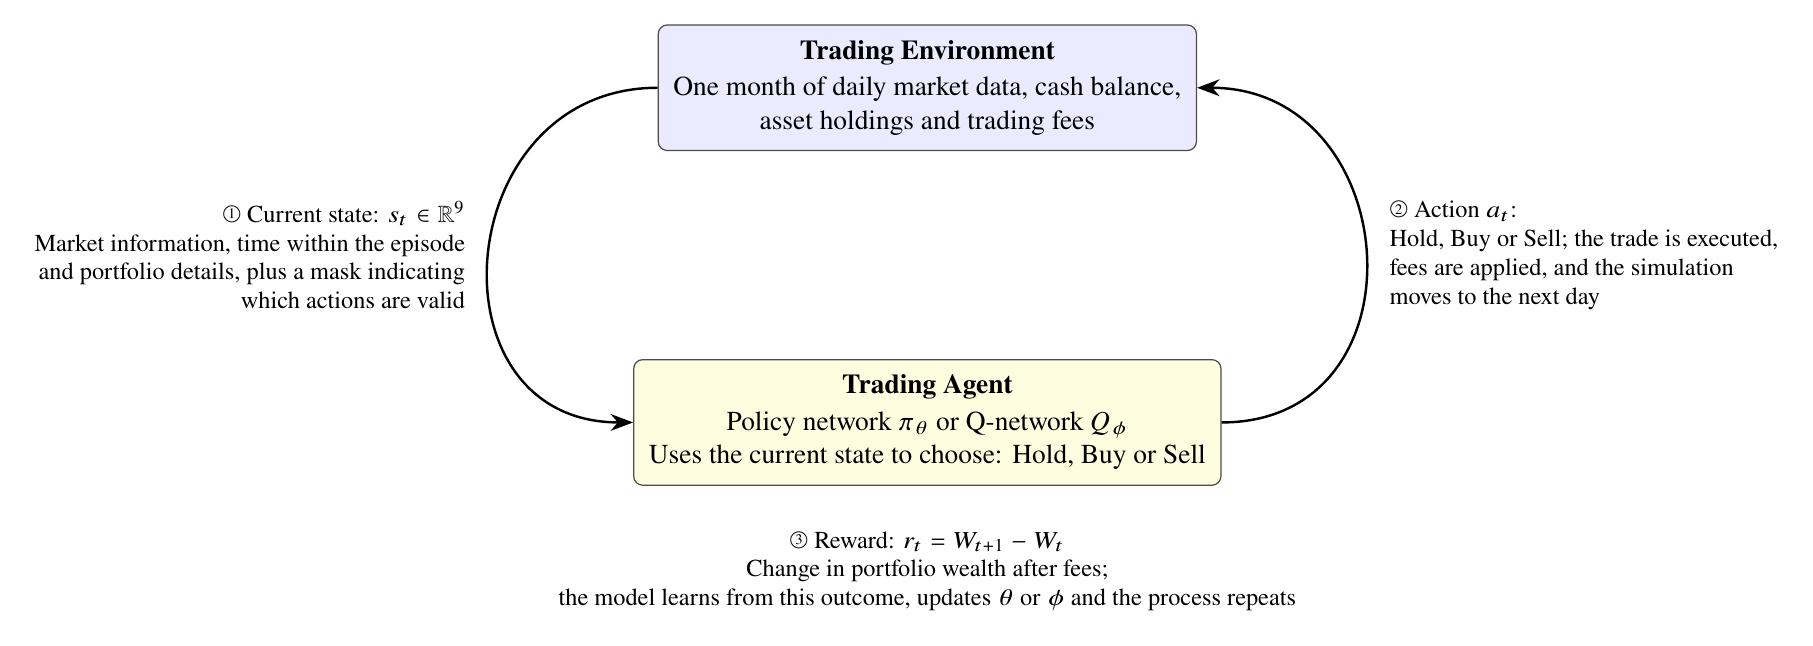
\includegraphics[width=0.9\textwidth]{media/media/image1_ch3.png}
  \caption[The agent--environment interaction loop for the trading MDP.]{The agent--environment interaction loop for the trading MDP. One cycle corresponds to one trading day.}
\end{figure}


To make the MDP formulation easier to understand, Table 3.2 compares the
main components of the trading task with those of a familiar
game-playing task, Flappy Bird, which was used initially to understand
Reinforcement Learning.

\addcontentsline{lot}{table}{\protect\numberline{3.2}{Mapping a popular game MDP to the portfolio trading MDP.}}
\textbf{Table 3.2: Mapping a popular game MDP to the portfolio trading
MDP.}

{\def\LTcaptype{none} % do not increment counter
\begin{longtable}[]{@{}
  >{\raggedright\arraybackslash}p{(\linewidth - 4\tabcolsep) * \real{0.2129}}
  >{\raggedright\arraybackslash}p{(\linewidth - 4\tabcolsep) * \real{0.3872}}
  >{\raggedright\arraybackslash}p{(\linewidth - 4\tabcolsep) * \real{0.3998}}@{}}
\toprule\noalign{}
\begin{minipage}[b]{\linewidth}\raggedright
\textbf{MDP component}
\end{minipage} & \begin{minipage}[b]{\linewidth}\raggedright
\textbf{Flappy Bird}
\end{minipage} & \begin{minipage}[b]{\linewidth}\raggedright
\textbf{Trading (this work)}
\end{minipage} \\
\midrule\noalign{}
\endhead
\bottomrule\noalign{}
\endlastfoot
State \emph{s\textsubscript{t}} & Bird\textquotesingle s position and
speed, together with the position of the next pipe & Market information
and the agent\textquotesingle s current portfolio position \\
\rowsep
Action \emph{a\textsubscript{t}} & Flap or do not flap & Hold, Buy, or
Sell \\
\rowsep
Reward \emph{r\textsubscript{t}} & Survival score based on how long the
bird remains in play & Change in portfolio wealth after trading fees \\
\rowsep
Episode \emph{τ} & One complete game session & One calendar month of
daily trading \\
\rowsep
Terminal rule & The game ends when the bird crashes or hits the ground &
The episode ends at the final trading day, with any remaining position
sold \\
\end{longtable}
}

This analogy also highlights a design principle used throughout the
project: as the Flappy Bird state contains the information relevant to
the next decision, the trading state includes the relevant information
available to the agent at each trading step, without being given future
information. Section 3.3 discusses the design of the trading state in
more detail.

\section{Episode Definition and Data Structure}

\subsection{Episode definition \texorpdfstring{\((\tau)\)}{()}}

Each episode \((\tau)\) represents one calendar month of daily closing
prices, from \(P_{0}\ to\ P_{T}\) \((P_{0},\ \ P_{1},\ldots,P_{T})\)
where \(T\) is typically between 18 and 23 trading days per month,
excluding public holidays when markets aren't open and weekends of
market inactivity \((T \approx 18 - 23)\). At the beginning of each
episode, the agent starts with cash and no asset holdings. It can then
trade throughout the month based on the available information. At the
end of the final trading day \(t\), any remaining position is
automatically sold. This ensures that no position is carried over from
one episode to the next.

\subsection{Independence of Trading Episodes}

For the purposes of the experiment, each monthly episode is treated as a
separate and independent trading period. This is similar to treating
each game session in Flappy Bird as a separate episode.

However, this is a simplification because market conditions in
consecutive months are not truly independent. For instance, events and
trends in one month do influence the market in the following month. The
resulting data are therefore not independent over time.

Modelling these temporal relationships in greater detail would require
time-series or partially observable approaches, which are outside the
scope of this project. The implications of this assumption are discussed
further in the conclusion\textbf{.}

\subsection{Choice of Episode Length}

Monthly episodes were selected to provide a balance between the length
of each trading period and the total number of training examples
available.

A single year of daily data provides approximately 12 monthly episodes
and around 250 daily trading decisions. Using eight years of data from
2018 to 2025 gives 96 monthly episodes and approximately 2,000 daily
transitions. These episodes are divided chronologically into 60 months
for training, 12 months for validation, and 24 months for the held-out
test period, as detailed in Chapter 4. The data are not shuffled, which
prevents information from later periods from being used during training
and helps avoid look-ahead leakage.

The same environment could also be adapted to shorter intervals, such
as minute-level data, without a fundamental change to its design, but
intraday trading is outside the scope of this study.

\subsection{Selection of the Historical Period}

The experiments use daily market data from 2018 to 2025 as a fixed
period. Earlier data, including data from 2016 and before, were not
included in the main experimental period because the study aims to
evaluate the learning algorithms under relatively recent and varied
market conditions. These selected periods contain a range of market
conditions, including relatively stable periods in 2018, the market
decline associated with the COVID-19 pandemic and its subsequent
recovery, the later period of increased inflation and interest rates,
and the war in Ukraine in 2022, which caused weaker market conditions.
As a result, the dataset is not limited to a single type of market
condition, providing a useful range for evaluating the behaviour of the
portfolios trading agents without extending the dataset into
substantially older market years.

Including older data, such as 2016 or earlier, would increase the
number of observations but could also introduce market conditions that
differ considerably from those in the selected period, such as older
microstructure and fee regimes. Earlier historical data are therefore
left to future work as an additional robustness test of how well the
trained agents generalise across market regimes.

It should also be noted that real financial markets are more complex
than any MDP and cannot be assumed to be fully observable. The MDP used
here is a simplified representation of the portfolio trading problem;
the information the agent cannot observe, and the consequences of this,
are discussed with the state representation in Section 3.3.

\section{State Representation Design}

In reinforcement learning, how information is presented to the agent
plays an important role in the quality of decisions it can learn. The
state representation must provide enough information for the agent to
understand the current situation and choose an appropriate action.

In this portfolio trading problem, this requires capturing information
about both the market and the agent\textquotesingle s own portfolio. The
agent needs to know how the asset has been moving, but it also needs to
know how much cash is available, whether it currently holds the asset,
whether that position is profitable, and how much time remains before
the trading period ends.

A state that leaves out important information can make it difficult for
the agent to learn effective strategies, even if the learning algorithm
is suitable for the task. This is because the agent can make decisions
only using the information provided. Therefore, the state representation
in this study was developed gradually by first examining simpler
representations and then adding information as needed to address
specific limitations of the previous representation.

The objective was not to create an unnecessarily complex state
representation with many variables, but to design a compact
representation containing all relevant information needed for
decision-making within the defined portfolio trading environment, while
avoiding features that simply duplicate information already available
from other variables

\subsection{Information Available to the Agent}

As discussed in Section 3.1, the state should see the whole by providing
the agent with information relevant to its decision, as the Flappy Bird
state does. In a trading environment, this information can be divided
into two halves: \textbf{the agent\textquotesingle s own portfolio} and
\textbf{the wider market}. These two areas behave very differently and
should therefore be considered separately when designing the state.

The first area is the agent\textquotesingle s own portfolio. This
includes information such as the amount of cash available, how much of
the asset it owns, what it paid to enter a trade position, and the time
remaining in the trading period. The agent controls this half; it is not
hidden or estimated, and it can be completely represented. Given the
sequence of the asset prices and the agent\textquotesingle s actions,
the portfolio can be updated directly using the trading environment's
rules.

The second area is the market. Here, complete information about the
market is impossible in principle and cannot be provided to the agent
because many factors affecting an asset's price are not directly
observable from the available price data. For example, the agent cannot
observe other market participants\textquotesingle{} decisions,
expectations, or intentions. Similarly, information such as news, market
sentiment, and macroeconomic events may influence prices without
appearing directly in the closing price at the end of the episode.

Adding more features calculated from past prices can give the agent
additional information about recent market behaviour, but it cannot
reveal everything happening in the market. The attainable goal is
therefore a state that is complete on the portfolio side and rich
enough on the market side: \textbf{the portfolio information can be
represented completely because the environment directly controls and
records it, whereas market information can only approximate the wider
market.} Whether the additional market features provide useful
information is ultimately an empirical question, which is considered
when evaluating the state representation later in the dissertation.

\subsection{Criteria for a Suitable Trading State}

It is tempting to design a state by asking which features look useful,
but this is a weak approach as it says nothing about whether the object
being trained is an MDP at all.

Before deciding on the final state representation, three conditions were
considered. These provide a basis for deciding whether the proposed
state contains the information required for the portfolio trading
problem.

\textbf{1. Reward measurability}

The reward should be calculable from information available to the agent
and the resulting transition. If the reward depends on information not
contained in the state or the transition, the agent is effectively being
evaluated using information it cannot observe.

The primary reward used in this study is the change in portfolio wealth,
\(r_{t} = W_{t + 1} - W_{t}\). The final state includes cash and asset
exposure as fractions of the initial capital, and these two features
combine to give the current wealth, so the reward can be calculated
from the observed transition \((s_{t},a_{t},s_{t + 1})\) with no hidden
portfolio variable. Section 3.5 defines the reward and shows this
derivation in full.

\textbf{2. Transition consistency}

The state should also contain enough information for the next state to
be determined from the current state, the selected action, the next
observed market price, and the trading environment rules.

This matters because the agent should not need to access hidden
historical variables to describe how its portfolio changes after an
action.

For example, the current portfolio exposure can be used to determine the
position's value, while the current unrealised profit/loss contains
information about the position\textquotesingle s entry price. Together
with the current price and the environment\textquotesingle s trading
rules, these quantities provide the information required to update the
portfolio after an action.

This keeps the state representation consistent with the defined trading
environment rather than requiring the environment to retrieve additional
portfolio history that is not represented in the state.

\textbf{3. Decision sufficiency}

The state should contain enough information for the agent to make a
decision based on the current trading situation without ambiguity. If
two different situations look identical to the agent but require
different actions, then the state is missing important information,
making the representation incomplete.

For example, consider the following two situations:

\begin{itemize}
\item
  the asset price has increased by 2\% today, and the agent does not
  hold the asset;
\item
  the asset price has increased by 2\% today, but the agent holds a
  position that is currently making a loss.
\end{itemize}

In both cases, the observed price movement is the same. However, the
most appropriate action may be different. In the first situation, the
agent may consider opening a position, whereas in the second, it may
consider reducing or closing its existing position to minimize its
losses.

The state representation must therefore include information about both
the market and the agent\textquotesingle s own portfolio.

\subsection{Development of the State Representation}

The state was developed in stages, starting from the smallest
representation that could describe a trading decision and adding
information only where the previous stage left the agent unable to
distinguish situations that require different actions. Table 3.4 at the
end of this section summarises the full progression.

The starting point was a price-only state,
\(s_{t}^{(0)} = \left\lbrack \Delta P_{t} \right\rbrack\), where
\(\Delta P_{t} = (P_{t} - P_{t - 1})/P_{t - 1}\) is the one-day return.
This is insufficient because the same market movement can occur in very
different trading situations. A positive daily return means one thing
when the agent holds nothing and may consider entering a position, and
another when it already holds a large position and may consider reducing
it. The agent cannot see its own portfolio.

Portfolio, position, and time information were therefore added in turn,
producing the following features:

\textbf{1. Normalised cash} \(\mathbf{(c}_{\mathbf{t}}\mathbf{)}\),
defined as \(c_{t} = C_{t}/C_{0}\), is the proportion of the initial
capital that remains available for future decisions. Using a normalised
value keeps the information consistent regardless of the starting
account size.

\textbf{2. Normalised exposure} \(\mathbf{(v}_{\mathbf{t}}\mathbf{)}\),
defined as \(v_{t} = h_{t}P_{t}/C_{0}\), is the current market value of
the open position relative to the initial capital. This replaces the raw
unit count \(h_{t}\) because the same number of units can represent a
small or large investment depending on the asset price. Together, the
two portfolio features recover the agent\textquotesingle s current
wealth as \(c_{t} + v_{t} = W_{t}/C_{0}\).

\textbf{3. Unrealised profit/loss}
\(\mathbf{(Pn}\mathbf{L}_{\mathbf{t}}\mathbf{)}\):

\[PnL_{t} = \frac{P_{t} - {\overline{P}}_{t}^{entry}}{{\overline{P}}_{t}^{entry}}\]

where \({\overline{P}}_{t}^{entry}\) is the average price at which the
current position was opened. This tells the agent whether its position
is in profit or loss --- two situations that look identical from the
market side but may call for different actions. Holding an asset after
a price increase may be profitable if it was bought at a lower price,
or losing money if the position was entered at a higher price before
the price declined.

\textbf{4. Episode clock} \(\mathbf{(\tau}_{\mathbf{t}}\mathbf{)}\),
defined as \(\tau_{t} = t/T\), where \(T\) is the total length of the
episode. A value close to 0 means the episode has just started, while a
value close to 1 means the forced close at the final trading day is
approaching. This matters because the same action can have different
consequences depending on when it is taken: buying early leaves the
position time to grow, whereas buying shortly before the episode ends
does not.

\subsection{Final State Representation}

Although the previous stages successfully introduced information about
the agent's portfolio and position, they provide limited understanding
of the broader market conditions. A trading decision should not depend
only on the most recent price change, as different market situations
exist, producing similar short-term movements.

For this reason, the agent also needs information that helps it
distinguish between market conditions: whether the asset is in a
short-term upward or downward trend, whether the market is stable or
highly volatile, and whether the current price is above or below its
recent average level. Additional market-related features are therefore
included to give the agent a more complete view of the trading
environment.

The final state representation is defined as:

\[\boxed{s_{t}^{(4)} = \left\lbrack \Delta P_{t},mom_{t},vol_{t},gap_{t},{rng_{t},\tau}_{t},c_{t},v_{t},PnL_{t} \right\rbrack \in \mathbb{R}^{9}}\]

The following variables were added:

\textbf{1. Momentum}

\[mom_{t} = \frac{P_{t} - P_{t - k}}{P_{t - k}}\]

where \(k = 5\) previous days (about one trading week). Momentum gives
the agent a longer view of the recent price direction, helping it
differentiate a temporary movement from a more consistent trend
developing over several timesteps.

\textbf{2. Volatility}

\[vol_{t} = \sigma\left( \Delta P_{t - k + 1},...,\Delta P_{t} \right)\]

where \(\sigma\) is the standard deviation of the last \(k = 5\) daily
returns. This helps the agent recognise differences in market
uncertainty: a 2\% price increase during a relatively stable period is
different from a 2\% increase during a period of large and frequent
price movements, which indicates a riskier situation.

\textbf{3. Price trend position}

\[gap_{t} = \frac{P_{t}}{MA_{m,t}(P)_{t}} - 1\]

where \({MA}_{m,t}(P) = \frac{1}{m}\sum_{i = 0}^{m - 1}P_{t - i}\) is
the simple moving average of the closing price over the previous
\((m = 20)\) days (about one trading month). A positive value means the
current price is above its recent average level and a negative value
means it is below, helping the agent identify potential trends or
deviations from normal price behaviour.

\textbf{4. Normalised Trading Range}

The normalised trading range is based on the Average True Range (ATR):

\[rng_{t} = \frac{ATR_{n,t}}{P_{t}}\]

The True Range at timestep \(t\) is
\(TR_{t} = \max\left( H_{t} - L_{t},\,\left| H_{t} - C_{t - 1} \right|,\,\left| L_{t} - C_{t - 1} \right| \right)\),
where \(H_{t}\) and \(L_{t}\) are the current high and low prices and
\(C_{t - 1}\) is the previous closing price. The ATR is the rolling
arithmetic mean of the last \((n = 14)\) True Range values (about two
trading weeks):

\[ATR_{n,t} = \frac{1}{n}\sum_{i = 0}^{n - 1}TR_{t - i}\]

The ATR therefore measures the size of recent price movement using the
asset's high, low, and closing prices, and dividing it by the current
price creates a normalised measure that can be compared across different
price levels.

The nine features and what each tells the agent are
summarised in Table 3.3.

\addcontentsline{lot}{table}{\protect\numberline{3.3}{Full State Definition}}
\textbf{Table 3.3: Full State Definition}

\emph{Table 3.3: The} \emph{nine-feature state representation
(s\textsubscript{t} ∈ ℝ\textsuperscript{9}) used in the main
experiments. C\textsubscript{0} denotes the initial cash,
h\textsubscript{t} the number of asset units held, and
W\textsubscript{t} = C\textsubscript{t} + h\textsubscript{t}
P\textsubscript{t} the portfolio wealth at time t. the mark-to-market
wealth. The feature timestep lengths are set to (k=5) for momentum and
volatility, (m=20) for the moving-average reference, and (n=14) for the
Average True Range.}

{\def\LTcaptype{none} % do not increment counter
\begin{longtable}[]{@{}
  >{\raggedright\arraybackslash}p{(\linewidth - 6\tabcolsep) * \real{0.0521}}
  >{\raggedright\arraybackslash}p{(\linewidth - 6\tabcolsep) * \real{0.1159}}
  >{\raggedright\arraybackslash}p{(\linewidth - 6\tabcolsep) * \real{0.2666}}
  >{\raggedright\arraybackslash}p{(\linewidth - 6\tabcolsep) * \real{0.5653}}@{}}
\toprule\noalign{}
\begin{minipage}[b]{\linewidth}\raggedright
\textbf{\#}
\end{minipage} & \begin{minipage}[b]{\linewidth}\raggedright
\textbf{Feature}
\end{minipage} & \begin{minipage}[b]{\linewidth}\raggedright
\textbf{Definition}
\end{minipage} & \begin{minipage}[b]{\linewidth}\raggedright
\textbf{What it tells the agent}
\end{minipage} \\
\midrule\noalign{}
\endhead
\bottomrule\noalign{}
\endlastfoot
\multicolumn{4}{@{}>{\raggedright\arraybackslash}p{(\linewidth - 6\tabcolsep) * \real{1.0000} + 6\tabcolsep}@{}}{%
\emph{\textbf{Market}}} \\
\rowsep
1 & \emph{ΔP\textsubscript{t}} & \emph{P\textsubscript{t}} -
\emph{P\textsubscript{t−1}}/ \emph{P\textsubscript{t−1}} & The most
recent price movement \\
\rowsep
2 & \emph{mom\textsubscript{t}} & \emph{P\textsubscript{t}} -
\emph{P\textsubscript{t−k}}/ \emph{P\textsubscript{t−k}} & whether that
recent price movement is part of a short-term trend \\
\rowsep
3 & \emph{vol\textsubscript{t}} &
\(\sigma\left( \Delta P_{t - k + 1},...,\Delta P_{t} \right)\) & how
much the asset price has been varying recently \\
\rowsep
4 & \emph{gap\textsubscript{t}} & \emph{P\textsubscript{t}} /
MA\emph{\textsubscript{m}}(P) − 1 & how far the current price is from
its recent average \\
\rowsep
5 & \emph{rng\textsubscript{t}} & ATR\emph{\textsubscript{n}}(P) /
\emph{P\textsubscript{t}} & The size of the recent price ranges, which
closing prices alone cannot show \\
\rowsep
\multicolumn{4}{@{}>{\raggedright\arraybackslash}p{(\linewidth - 6\tabcolsep) * \real{1.0000} + 6\tabcolsep}@{}}{%
\emph{\textbf{Portfolio}}} \\
\rowsep
6 & \emph{c\textsubscript{t}} & \emph{C\textsubscript{t}} /
\emph{C\textsubscript{0}} & how much of the initial cash remains
available as cash \\
\rowsep
7 & \emph{v\textsubscript{t}} & \emph{h\textsubscript{t}}
\emph{P\textsubscript{t}} / \emph{C\textsubscript{0}} & The current
value of the open position relative to the initial capital \\
\rowsep
\multicolumn{4}{@{}>{\raggedright\arraybackslash}p{(\linewidth - 6\tabcolsep) * \real{1.0000} + 6\tabcolsep}@{}}{%
\emph{\textbf{Position}}} \\
\rowsep
8 & \emph{PnL\textsubscript{t}} & (\emph{P\textsubscript{t}} −
\emph{P̄\textsubscript{tentry}}) / \emph{P̄\textsubscript{tentry}} &
whether the open positions are in profit or loss \\
\rowsep
\multicolumn{4}{@{}>{\raggedright\arraybackslash}p{(\linewidth - 6\tabcolsep) * \real{1.0000} + 6\tabcolsep}@{}}{%
\emph{\textbf{Time}}} \\
\rowsep
9 & \emph{τ\textsubscript{t}} & \emph{t} / \emph{T} ∈ {[}0, 1{]} & how
much time remains before the trading episode ends \\
\end{longtable}
}

\subsection{Feature Redundancy and Excluded Information}

The state was not designed by adding every potentially useful market
indicator. Features were included only where they provide information
that cannot already be recovered from the other variables in the state.

This is important because adding a feature that simply repeats existing
information increases the size of the input without providing the agent
with anything new.

The following features were excluded:

\textbf{1. Running portfolio return}

For example, the portfolio\textquotesingle s current return relative to
its starting capital\\
does not need to be included as a separate feature because it can
already be calculated from the normalised cash and asset exposure as
\(c_{t} + v_{t}\). Adding it would duplicate information already
available in the state.

\textbf{2. Raw position size}

The raw number of units held, \(h_{t}\), is also not included in the
final state. The financial value of the position is more directly
represented by:

\[v_{t} = \frac{h_{t}P_{t}}{C_{0}}\]

This provides information about the actual exposure rather than only the
number of units.

\textbf{3. Raw asset price}

The raw asset price is also not required as a separate feature. The
state instead uses returns and normalised values, which describe price
movements without depending on the standard price level.

The general principle is therefore to include features that provide
useful information while avoiding variables that can already be
reconstructed from information available elsewhere in the state.

\subsection{The Risk-Aware Extension: Drawdown State}

The main state representation contains the information needed for the
change in wealth reward. However, it does not describe the history of
the portfolio's losses: current wealth alone does not show how the
portfolio reached its current value. For example, two portfolios can
have exactly the same wealth at the current timestep but may have
followed very different paths:

\begin{itemize}
\item
  one portfolio may have increased steadily over time;
\item
  another may have suffered a large loss before recovering to the same
  level.
\end{itemize}

To address this, an additional feature representing portfolio drawdown
is introduced as a separate risk-aware extension:

\[dd_{t} = \frac{\max_{u \leq t}W_{u} - W_{t}}{\max_{u \leq t}W_{u}}\]

where \(dd_{t}\) represents the current decline in portfolio wealth from
the highest wealth level reached so far during the episode.

A value of zero means that the portfolio is currently at its highest
wealth level reached so far in the episode. A larger value indicates
that the portfolio has fallen further below its previous peak.

For this reason, drawdown is treated separately from the main state
representation. This makes it possible to evaluate whether explicitly
providing information about portfolio loss history affects the
agent\textquotesingle s behaviour and performance.

The resulting risk-aware state is therefore:

\[s_{t}^{risk} \in R^{10}\]

where:

\[s_{t}^{risk} = \left\lbrack s_{t},dd_{t} \right\rbrack\]

Since the original state \(s_{t}\) contains nine features, adding
drawdown produces a \textbf{ten-dimensional} risk-aware state.

\subsection{Feature Calculation and Information Timing}

The timing of feature calculation matters because the agent should
receive only the information available when making its trading decision.
Using future information would give the agent an unfair advantage and
could lead to overly optimistic results.

For this reason, the market features are calculated using information
available at or before timestep \((t)\). The current price and past
prices can be used to create the state, but the agent must not use
future prices when it decides its action \((a_{t})\).

The same principle applies to the features that use historical windows:
momentum uses the previous \((k = 5)\) timesteps, the moving average the
previous \((m = 20)\) prices, and the normalised trading range the
\((n = 14)\)-day ATR, as reported in Table 3.3.

Therefore, each state is based only on information that is available at
the time the decision is made. This prevents future market information
from entering the agent\textquotesingle s observation and helps avoid
\textbf{look-ahead bias}, where a model appears to perform well because
it has indirectly been given information that would not have been
available during actual trading.

\subsection{State Representation Limitations}

Although the final state representation gives the agent a wider range of
information, the trading environment is still a simplified
representation of a real financial market.

The agent does not have access to several types of information that can
influence real-world trading decisions, including:

\begin{itemize}
\item
  order flows;
\item
  market sentiment;
\item
  financial news;
\item
  macroeconomic conditions;
\item
  relationships between the asset and other financial assets.
\item
  The actions and intentions of large financial institutions.
\end{itemize}

These limitations mean that the state should not be interpreted as a
complete description of the real financial market. Because this relevant
information cannot be represented in the environment, it is better to
describe this as a \emph{\textbf{partially observable Markov decision
process (POMDP)}} rather than a fully observable one.

However, this dissertation does not aim to replicate every aspect of
real-world financial markets. The purpose is to compare and evaluate
reinforcement learning algorithms within a controlled trading
environment for an asset.

The proposed state representation therefore provides sufficient
information for the defined task and can be \textbf{considered complete
with respect to} \textbf{the information used by the defined trading
environment}, which includes recent market behaviour, the current
portfolio position, the performance of its current position, and the
amount of time remaining in the trading period, while acknowledging that
the model does not capture all factors present in real-world trading.

\subsection{Summary}

The final state was not selected because it contained a particular
number of variables, but because its components collectively describe
the market conditions, portfolio exposure, position performance, and
remaining trading episode available within the defined environment.
Table 3.4 summarises the design progression and the limitation each
stage resolved.

\addcontentsline{lot}{table}{\protect\numberline{3.4}{The staged development of the state representation. Each stage resolves the limitation named in the row above it.}}
\emph{Table 3.4: The staged development of the state representation.
Each stage resolves the limitation named in the row above it.
ΔP\textsubscript{t} is the one-step return, c\textsubscript{t} cash and
v\textsubscript{t} exposure as fractions of initial capital,
h\textsubscript{t} the units held, τ\textsubscript{t} the episode clock
and dd\textsubscript{t} the fall from peak wealth.}

{\def\LTcaptype{none} % do not increment counter
\begin{longtable}[]{@{}
  >{\raggedright\arraybackslash}p{(\linewidth - 4\tabcolsep) * \real{0.1007}}
  >{\raggedright\arraybackslash}p{(\linewidth - 4\tabcolsep) * \real{0.3148}}
  >{\raggedright\arraybackslash}p{(\linewidth - 4\tabcolsep) * \real{0.5665}}@{}}
\toprule\noalign{}
\begin{minipage}[b]{\linewidth}\raggedright
\textbf{Stage}
\end{minipage} & \begin{minipage}[b]{\linewidth}\raggedright
\textbf{State}
\end{minipage} & \begin{minipage}[b]{\linewidth}\raggedright
\textbf{Limitation addressed by the next stage}
\end{minipage} \\
\midrule\noalign{}
\endhead
\bottomrule\noalign{}
\endlastfoot
\emph{S\textsubscript{0}} & {[}\emph{ΔP\textsubscript{t}}{]} & The agent
can observe recent price movement but has no information about its own
portfolio. It cannot tell whether it already holds the asset, or whether
it has enough cash to open a position. \\
\rowsep
\emph{S\textsubscript{1}} & {[}\emph{ΔP\textsubscript{t}},
\emph{c\textsubscript{t}}, \emph{h\textsubscript{t}}{]} & The agent now
knows its available cash and the number of units it holds but not what
they are worth. For example, ten units could represent a small or large
investment depending on the asset price. \\
\rowsep
\emph{S\textsubscript{2}} & {[}\emph{ΔP\textsubscript{t}},
\emph{c\textsubscript{t}}, \emph{v\textsubscript{t}},
\emph{PnL\textsubscript{t}}{]} & The agent can now determine the value
of its position and tell whether its in profit or loss, but it does not
know where it stands in the month. A position opened at the beginning of
the month can therefore appear identical to one made immediately before
the required closing of the position at the end of the month. \\
\rowsep
\emph{S\textsubscript{3}} & {[}\emph{ΔP\textsubscript{t}},
\emph{c\textsubscript{t}}, \emph{v\textsubscript{t}},
\emph{PnL\textsubscript{t}}, \emph{τ\textsubscript{t}}{]} & The
agent\textquotesingle s own circumstances are now fully represented, but
its view of the market is still limited to the most recent price return.
It cannot tell a stable trend from a reversal, or between relatively
stable and highly volatile conditions. \\
\rowsep
\emph{S\textsubscript{4}} & adds momentum, volatility, distance from
trend, and daily range (Table 3.3) & The state provides a broader
representation of the market while retaining the portfolios information.
It is treated as the main state used in the experiments. \\
\rowsep
\emph{S\textsubscript{risk}} & adds \emph{dd\textsubscript{t}} & Adds
information about the portfolio\textquotesingle s previous losses from
its highest wealth level. Required when the experiment considers risk
history \\
\end{longtable}
}

The separate tenth feature, drawdown, is used only for the risk-aware
experiments described in Section 3.3.6.

The main state representation provides the basis for defining the
available actions and applying the reinforcement learning algorithms
described in the following sections.

\section{Action Space Design}

\subsection{Overview}

The action space defines the choices available to the trading agent at
each timestep. Its design matters because it determines how the agent
interacts with the market and what its learned policy means.

A poorly designed action space can introduce unnecessary complexity or
create unrealistic trading behaviour. For example, allowing the agent to
choose any number of shares to buy or sell adds learning challenges: the
agent must simultaneously learn when to trade\textbf{,} which direction
to take\textbf{,} and how much to trade. This can make it difficult to
determine whether poor performance results from an ineffective trading
strategy or from difficulty learning appropriate position sizes.

To keep the focus on the trading decisions made by the reinforcement
learning algorithms, this study uses \textbf{a simplified discrete
action space}. The agent decides on the action (trading direction),
while the environment determines the amount traded.

This separates the trading problem into two decisions:

\begin{enumerate}
\def\labelenumi{\arabic{enumi}.}
\item
  \textbf{When and in which direction to trade} --- this is the trading
  policy being learned by the reinforcement learning algorithm.
\item
  \textbf{How much capital to trade} --- this is fixed by the
  environment and treated as an experimental setting.
\end{enumerate}

This approach keeps the action space simple and makes it easier to
compare the learning algorithms on the same portfolio trading task. It
also means that differences in performance can be interpreted mainly in
terms of the agents\textquotesingle{} ability to learn trading
decisions, rather than their ability to learn position sizing.

\subsection{Trading Actions and Trade Size}

The action space is defined as \(A = \left\{ 0,1,2 \right\}\), where
action 0 \textbf{holds} the current position, action 1 \textbf{buys} a
fixed amount, and action 2 \textbf{sells} a fixed amount. At each
timestep, the agent selects one of these three actions using the
information available in the current state.

The \textbf{hold} action leaves the portfolio unchanged. No transaction
takes place: the available cash and the number of units held remain the
same, and no transaction fee is charged. This allows the agent to remain
in its current position when it does not consider buying or selling to
be appropriate.

The \textbf{buy} and \textbf{sell} actions change the
agent\textquotesingle s exposure to the asset by a fixed monetary
amount:

\[\Delta = f\,C_{0}\]

where \(C_{0}\) is the initial capital and \(f\) is the fraction of that
capital allocated to one transaction. A fixed monetary amount is used
rather than a fixed number of shares because the cost of one share
depends heavily on the price level: buying one share of an asset priced
at \pounds 10 is a small investment, while buying one share priced at
\pounds 1,000 is a large one, even though both would be described as
buying one share. Fixing the monetary size keeps every trade at the same
proportion of the initial capital throughout the dataset, regardless of
the asset price.

The fraction \(f\) is treated as an experimental setting rather than a
fixed design constant. It is selected using the validation data before
the final experiments, as reported in Section 5.3.

The number of units bought or sold at price \(P_{t}\) is:

\[\Delta h_{t} = \pm\frac{\Delta}{P_{t}}\]

with the positive sign for a buy and the negative sign for a sell, and
with fractional ownership allowed, similar to a real-world portfolio. A
sell is valid only when the agent holds enough units for the transaction.
Because the trade size is fixed, the agent can build or reduce its
position gradually over several decisions while still operating within a
simple three-action framework.

\subsection{Action Constraints}

Although the agent has three possible actions, some actions may not be
possible at a particular timestep because of the current portfolio
position.

For example:

\begin{itemize}
\item
  the agent cannot buy if it does not have enough available cash;
\item
  the agent cannot sell if it does not hold enough of the asset to
  withdraw.
\end{itemize}

To handle these situations, the environment uses a \textbf{legal action
mask}. The mask does not provide any additional market information to
the agent. It simply indicates which actions can be carried out given
the current portfolio status.

The mask is represented as
\(M_{t} = \left\lbrack m_{\text{hold}},m_{\text{buy}},m_{\text{sell}} \right\rbrack \in \left\{ 0,1 \right\}^{3}\),
where \(M_{t}(a) = 1\) indicates that action \(a\) is available and
\(M_{t}(a) = 0\) indicates that it is not.

The availability of each action is determined from the portfolio state:

\begin{itemize}
\item
  available cash determines whether a \textbf{buy} action can be carried
  out;
\item
  the current asset holding determines whether a \textbf{sell} action
  can be carried out;
\item
  \textbf{hold} remains available throughout the episode.
\end{itemize}

Because the mask is derived directly from information already in the
portfolio state, it is not treated as an additional feature of the state
representation. Instead, it acts as a constraint on the agent,
preventing it from selecting actions the environment cannot execute.

\subsection{Transaction Costs}

A transaction fee of \(c = 0.05\%\) is charged whenever the agent
carries out a buy or sell action, so a transaction of value \(\Delta\)
incurs a fee of \(\Delta c\). The same fee calculation is applied to
both purchases and sales.

Including transaction costs matters because it prevents the agent from
overly buying and selling repeatedly. Without these fees, the agent
could benefit from making many trades even when price movements are very
small, making frequent trading appear more profitable than it would be
in practice.

The inclusion of fees therefore introduces a basic cost of trading into
the environment and provides a more realistic basis for evaluating
learned trading strategies.

\subsection{Relationship Between the State and Actions}

The action space was designed to match the state representation of
Section 3.3. Deciding whether to buy or sell depends on the
agent\textquotesingle s current exposure, its available cash, whether an
existing position is in profit or loss, the time remaining in the
episode, and the current market conditions --- exactly the information
the state provides. The agent decides whether to hold, buy, or sell,
while the environment determines the amount traded and prevents invalid
actions from being carried out.

\section{Reward Function Design}

\subsection{Purpose of the Reward Function}

The reward function tells the reinforcement learning algorithm how well
it performed after taking an action and guides the agent toward more
desirable actions. Unlike supervised learning, where the model is given
the correct answer, the agent learns by taking actions and receiving
feedback on the results of those actions.

In a trading environment, the reward function needs to accurately
reflect the actual objective of the investment strategy. If it is poorly
designed, the agent may learn behaviours that are not desirable, such as
trading too frequently, taking unnecessary risks, or performing well
during training but poorly under realistic conditions.

The main goal of this dissertation is to investigate whether
reinforcement learning algorithms can learn profitable trading
strategies for the selected asset while accounting for transaction
costs. For this reason, the primary reward is based on the
\textbf{change in portfolio wealth} from one timestep (trading day) to
the next.

\subsection{Wealth-Based Reward}

The main reward used in this study is based on the change in the
portfolio\textquotesingle s total value:

\[r_{t} = W_{t + 1} - W_{t}\]

where portfolio wealth at timestep \(t\) is given by:

\[W_{t} = C_{t} + h_{t}P_{t}\]

Here:

\begin{itemize}
\item
  \(C_{t}\) represents the cash available in the portfolio;
\item
  \(h_{t}\) represents the number of asset units held;
\item
  \(P_{t}\) represents the current asset price.
\end{itemize}

The reward therefore measures how much the portfolio\textquotesingle s
total value changes from one timestep (trading day) to the next after
the agent\textquotesingle s action.

A \textbf{positive reward} means the portfolio increased in value, while
a \textbf{negative reward} means it decreased. This gives the agent a
direct measure of the financial outcome of its decisions.

\subsection{Including Transaction Costs in the Reward}

Transaction fees are included when calculating the reward so that the
result reflects the actual cost of carrying out a trade.

When a buy or sell action is taken at timestep \(t\), the portfolio
value is updated after the transaction fee is deducted:

\[W_{t + 1} = C_{t + 1} + h_{t + 1}P_{t + 1} - Fees\]

The reward is then calculated from the resulting change in portfolio
wealth. This means that the agent is rewarded or penalised based on the
value of the portfolio \textbf{after trading costs have been taken into
account}.

\subsection{Wealth Change As the Primary Reward}

The change in portfolio wealth was chosen as the main reward for several
reasons.

First, it directly reflects the main objective of the trading strategy:
\textbf{increasing the value of the portfolio}. This also makes the
reward closely related to the metric used to evaluate investment
performance in the real world.

Second, it satisfies the requirements of the MDP defined in Section 3.2
because the reward can be obtained from portfolio information in the
state representation.

The current portfolio wealth can be recovered from the cash and exposure
features in the state representation:

\[c_{t} + v_{t} = \frac{W_{t}}{C_{0}}\]

Therefore, the change in wealth can be written as:

\[W_{t} = C_{0}\left\lbrack \left( c_{t} + v_{t} \right) \right\rbrack\]

\[r_{t} = C_{0}\left\lbrack \left( c_{t + 1} + v_{t + 1} \right) - \left( c_{t} + v_{t} \right) \right\rbrack\]

This shows that the reward depends only on the observed transition
\(\left( s_{t},a_{t},s_{t + 1} \right)\), without requiring additional
information unavailable to the agent.

\subsection{Risk-Aware Reward Extension}

Although the main objective is to increase portfolio wealth, focusing
only on returns may encourage the agent to take more risk than desired.
For example, a strategy may achieve a high final return but experience
large losses along the way, which is not a desirable trading behaviour.

Therefore, a risk-adjusted reward that accounts for changes in portfolio
drawdown is considered as an additional experimental condition:

\[r_{t}^{\mathrm{risk}} = \Delta W_{t} - \lambda\, C_{0}\, \Delta dd_{t}\]

where:

\begin{itemize}
\item
  \(\Delta W_{t}\) is the change in portfolio wealth;
\item
  \(\Delta dd_{t}\) is the increase in portfolio drawdown at step \(t\)
  (and is zero when drawdown does not rise);
\item
  \(C_{0}\) is the initial capital;
\item
  \(\lambda\) controls the penalty applied to increases in drawdown.
\end{itemize}

Drawdown measures how far the current portfolio wealth has fallen from
the highest level reached so far:

\[dd_{t} = \frac{\max_{u \leq t}W_{u} - W_{t}}{\max_{u \leq t}W_{u}}\]

where \(W_{t}\) is the portfolio wealth at time \(t\), and \(W_{u}\) is the
wealth at any earlier time \(u\) up to \(t\).
\(\max_{u \leq t}W_{u}\) is therefore the highest wealth reached so far
in the episode.

\(\Delta dd_{t}\) is therefore the increase in drawdown from one trading
day to the next. Multiplying it by the initial capital \(C_{0}\) keeps
the reward in dollars, so a penalty of \(\lambda = 0\) lets the
wealth-change reward remain the same, while a larger \(\lambda\)
discourages actions that worsen the drawdown.

However, this reward requires access to the
portfolio\textquotesingle s previous performance because the previous
highest wealth reached up to time \(t\) must be known in order to
calculate drawdown.

For this reason, the risk-aware reward is used only with the
\textbf{risk-aware state extension} described in Section 3.3.6. This
ensures that the information needed to calculate the reward is available
to the agent.

The wealth-change reward remains the main reward used in the baseline
experiments. The risk-aware version is treated separately so that the
effect of explicitly including information about portfolio loss history
can be examined.

\subsection{Limitations of the Reward Function}

Although the wealth-change reward provides a clear and direct measure of
trading performance, it does not capture every aspect of a desirable
trading strategy.

For Example, it does not directly penalise:

\begin{itemize}
\item
  large falls in portfolio value;
\item
  unstable performance in returns;
\item
  high levels of volatility.
\end{itemize}

A strategy could therefore achieve a strong overall return while
experiencing substantial losses during the trading period. The
limitations are addressed by the risk-aware reward in Section 3.5.5 by
adding a penalty when drawdown increases.

However, adding more objectives changes the learning problem and what
the agent is being trained to optimise. This can make comparisons
between algorithms less straightforward because improvements may result
from the different reward definition rather than from the learning
algorithm itself.

Therefore, the \textbf{wealth-change reward is used as the common
baseline}, while the risk-aware reward is considered separately as an
additional experiment.

\section{Objective Function}

The objective function describes what the reinforcement learning
algorithms are trying to achieve during training. In this study, the aim
is to learn a trading policy that produces the highest possible expected
return over each trading episode.

The reward function introduced in Section 3.5 measures the result of an
individual decision, while the objective function extends this idea by
combining the rewards received throughout the episode.

\subsection{Episode Return}

An episode/trajectory can be represented by the sequence:

\[\tau = \left( s_{0},a_{0},r_{0},s_{1},a_{1},r_{1},\ldots,s_{T} \right)\]

where \(s_{t}\) is the state observed at timestep \(t\),

\(a_{t}\)is the action selected by the agent, and

\(r_{t}\) is the reward resulting from that action.

The episode contains \(T\) trading decisions and ends when it reaches
the final market observation. Any position that remains open at this
point is then closed according to the rules of the trading environment.

The total discounted return from the beginning of the episode is:

\[G_{0} = \sum_{t = 0}^{T - 1}\gamma^{t}r_{t},\]

Where \(\gamma \in (0,1\rbrack\) is the discount factor.

The same calculation can be made from any point within the episode. The
return from timestep \(t\), commonly referred to as the
\textbf{reward-to-go}, is:

\[G_{t} = \sum_{t' = t}^{T - 1}\gamma^{t' - t}r_{t'}.\]

This represents the rewards expected from the current timestep onwards.
It is particularly relevant to the REINFORCE implementation because it
associates an action with the rewards that follow it, rather than
assigning the episode\textquotesingle s total return to every action
taken in that episode.

A discount factor of \(\gamma = 0.99\) is used throughout the
experiments. The trading episodes contain approximately 18--23 daily
observations, so this value results in relatively mild discounting over
the length of an episode: \({0.99}^{20} \approx 0.82\), so a reward
received near the end of the monthly episode still contributes around
82\% of its original value to the discounted return.

Using \(\gamma = 0.99\), therefore, maintains the standard
reinforcement-learning formulation for discounted returns while still
ensuring the objective is maximising end-of-month wealth.

\subsection{Expected Return}

The outcome of a single trading episode is not enough to judge the
quality of a policy because each episode can reflect different market
conditions experienced during that month. For instance, a policy that
performs well in one month may not perform equally well in another.
Therefore, the objective is defined using the expected returns the
policy earns across different trading episodes.

The policy is represented by

\[\pi_{\theta}\left( a|s \right),\]

where \(\theta\) represents the trainable parameters of the policy
network. For a given state, the policy assigns probabilities to the
available actions, allowing the agent to choose between Buy, Hold, and
Sell.

\[\pi_{\theta}\left( a_{t} \mid s_{t} \right) = \begin{bmatrix}
P\left( a_{t} = \text{Hold} \mid s_{t} \right) \\
P\left( a_{t} = \text{Buy} \mid s_{t} \right) \\
P\left( a_{t} = \text{Sell} \mid s_{t} \right)
\end{bmatrix}\]

The expected return is defined as:

\[J(\theta) = \mathbb{E}_{\tau \sim p_{\theta}(\tau)}\left\lbrack G_{0}(\tau) \right\rbrack\]

The learning objective is therefore:

\[\theta^{*} = \arg{\max_{\theta}{J(\theta)}}.\]

In simple terms, the aim is not for the agent to find a policy that
performs well in only one trading period. Instead, the agent should
learn policy parameters that produce good, expected performance across
the different monthly market episodes used during training.

The policy parameters affect the objective only through the actions the
agent selects: changing \(\theta\) changes the probabilities of choosing
Buy, Hold, or Sell in each state, and these decisions affect the
portfolio and, in turn, the rewards collected over the episode.

\subsection{Objective and the Trading Environment}

The formulation above also separates the trading
environment\textquotesingle s role from the learning
algorithm\textquotesingle s. The environment determines the market data,
the current portfolio state, the transaction costs, which actions are
currently valid, the resulting portfolio wealth, the reward, and whether
the episode has ended. The learning algorithm determines only how the
agent updates its policy or value function using that experience.

This separation is important for comparing the different learning
approaches in this dissertation. \textbf{REINFORCE, DQN, and PPO} use
the same state representation, action space and masking, market data,
and reward function, so differences in their results stem from how they
learn rather than from the conditions they operate under.

\section{REINFORCE: Monte-Carlo Policy Gradient}

REINFORCE is the first policy-gradient method used in this study. Unlike
value-based methods, which estimate how useful different actions are in
a given state, \textbf{REINFORCE directly learns a policy} that gives
probabilities to the available actions.

It provides a useful baseline because its main idea is straightforward.
The agent selects actions according to its current policy, observes the
resulting rewards, and then adjusts the policy so actions can lead to
better returns in the future.

\subsection{Policy Representation}

The policy is represented by a neural network with trainable parameters
\(\theta\). Given the current state \(s_{t}\), the network produces one
output, or logit, for each of the three possible actions
\(\left\{ \text{Buy},\ \text{Hold},\ \text{Sell} \right\}\).
Actions that are not permitted at the current timestep using the action
mask described in Section 3.4 are removed. The remaining logits are then
passed through a SoftMax function to produce the policy probabilities
\(\pi_{\theta}\left( a_{t}|s_{t} \right)\).

During training, the agent samples an action from this probability
distribution. This lets it try different actions and explore alternative
trading decisions rather than always choosing the action with the
highest probability.

During evaluation, the agent selects the valid action with the highest
probability without exploring.

The policy network used in this study has \textbf{two hidden layers,
each with 128 units}, and uses the hyperbolic tangent \(\tanh\) as the
activation function. The final layer produces one output for each of the
three available actions.

\subsection{Deriving the Policy-Gradient Objective}

The objective introduced in Section 3.6 is an expected return over
trading episodes:

\[J(\theta) = \mathbb{E}_{\tau \sim p_{\theta}(\tau)}\left\lbrack G_{0}(\tau) \right\rbrack.\]

To improve the policy, the learning algorithm needs to determine how a
small change to the policy parameters \((\theta)\) affects this expected
return. This requires calculating the gradient:

\[\nabla_{\theta}J(\theta).\]

The difficulty is that the probability of a complete trading episode
\(p_{\theta}(\tau)\) depends on the initial state, the actions selected
by the policy, and the resulting environment transitions
\(\left( s_{0},a_{0},r_{1},s_{1},a_{1},r_{2},...,s_{T} \right)\). It can
be written as:

\[p_{\theta}(\tau) = \rho\left( s_{0} \right)\prod_{t = 0}^{T - 1}\pi_{\theta}\left( a_{t}|s_{t} \right)P\left( s_{t + 1}|s_{t},a_{t} \right),\]

where \(\rho\left( s_{0} \right)\) represents the probability
distribution of initial states and

\(P\left( s_{t + 1}|s_{t},a_{t} \right),\) represents the environment's
transition to the next state \(s_{t + 1}\) given the current state and
action \({(s}_{t},a_{t})\).

The important point is that the policy parameters \((\theta)\) affect
the action probabilities\(\ \pi_{\theta}\left( a_{t}|s_{t} \right)\) but
not the market transition process. REINFORCE therefore does not need to
model this market transition explicitly, just the action probabilities.

So, we use the likelihood-ratio identity, which provides a way of
expressing the gradient \(\nabla_{\theta}J(\theta)\) using the
probability of the sampled episodes \(p_{\theta}(\tau)\):

\[\nabla_{\theta}p_{\theta}(\tau) = p_{\theta}(\tau)\nabla_{\theta}{\log p}_{\theta}(\tau).\]

The policy gradient can then be expressed as:

\[\nabla_{\theta}J(\theta) = \mathbb{E}_{\tau\sim p_{\theta}}\left\lbrack \nabla_{\theta}{\log p}_{\theta}(\tau){\ G}_{0}(\tau) \right\rbrack.\]

Since only the policy terms depend on \((\theta)\), this simplifies to

\[\nabla_{\theta}J(\theta) = \mathbb{E}_{\tau{\sim p}_{\theta}}\left\lbrack \sum_{t = 0}^{T - 1}\nabla_{\theta}{\log\pi}_{\theta}\left( a_{t}|s_{t} \right)G(\tau) \right\rbrack.\]

This is the basic policy-gradient expression REINFORCE uses in this
study.

In simple terms, the equation adjusts the probability of an action based
on the outcome that follows it. Actions resulting in higher returns are
encouraged by increasing their probability, while actions associated
with lower returns are made less likely.

\subsection{Reward-to-Go}

Using the complete episode return \(G(\tau)\) for every action is
inefficient because an action taken at time \(t\) cannot influence
rewards already received before that time. REINFORCE therefore weights
each action by the reward-to-go \(G_{t}\) defined in Section 3.6, so
only rewards from time \(t\) onwards are used when evaluating the
outcome associated with that decision.

The policy gradient can therefore be written as:

\[\nabla_{\theta}J(\theta) = \mathbb{E}\left\lbrack \sum_{t = 0}^{T - 1}\nabla_{\theta}{\log\pi}_{\theta}\left( a_{t}|s_{t} \right)G_{t} \right\rbrack.\]

where \(\nabla_{\theta}{\log\pi}_{\theta}\left( a_{t}|s_{t} \right)\)
is the direction in which the policy\textquotesingle s action
probability changes, and \(G_{t}\) is the return obtained after taking
action \(a_{t}\). This links each decision directly to the rewards that
followed it.

\subsection{Monte-Carlo Estimation}

The expectation \(\mathbb{E}\) in the policy-gradient equation cannot
normally be calculated because the full distribution of possible market
trajectories is unknown. REINFORCE therefore uses a Monte Carlo
approach: the agent interacts with the trading environment and uses the
resulting episodes to estimate the gradient.

For \(N\) sampled episodes, the gradient can be approximated as:

\[\nabla_{\theta}J(\theta) \approx \frac{1}{N}\sum_{n = 1}^{N}{\sum_{t = 0}^{T_{n} - 1}\nabla_{\theta}}{\log\pi}_{\theta}\left( a_{t}^{(n)}|s_{t}^{(n)} \right)G_{t}^{(n)}.\]

The superscript \(n\) represents the number of the sampled episode.

The gradient is therefore estimated from the average experience
collected from the sampled episodes.

This is why REINFORCE is described as a \textbf{Monte-Carlo
policy-gradient method}: The method does not require the agent to know
in advance how the market will move or to build a separate model of
future price changes. Instead, it learns how to estimate the expected
policy gradient from complete sampled episodes produced by its
interaction with the environment.

\subsection{Loss Function Used for Training}

Most neural-network frameworks are designed to minimise a loss function,
while reinforcement learning is to maximise expected rewards
\(J(\theta)\). The policy-gradient objective can therefore be written as
a loss by introducing a negative sign:

\[L(\theta) = - \frac{1}{N}\sum_{n = 1}^{N}{\sum_{t = 0}^{T_{n} - 1}{\log\pi}_{\theta}}\left( a_{t}^{(n)}|s_{t}^{(n)} \right)G_{t}^{(n)}.\]

The negative sign changes the original maximisation problem into a
minimisation problem that can be handled by the PyTorch optimiser.

The logarithm appears as a direct result of the likelihood-ratio
derivation above; it is not an additional trading assumption.

The implementation uses the \textbf{Adam optimiser}~\cite{kingma2015adam}
with a learning rate of \(10^{- 3}\).

During implementation, the sampled returns may also be normalised before
being used in the update. This helps control the gradient magnitude
across different training batches and can improve numerical stability.

\subsection{Strengths and Limitations}

REINFORCE is a suitable baseline for this project because its
formulation is relatively straightforward: it directly learns the
policy and does not require a separate model of the market, so
performance differences against more advanced algorithms are easier to
interpret.

Its main limitation is that \textbf{its gradient estimates can have high
variance} because they depend completely on episode returns, and
different episodes can produce very different outcomes even in similar
trading situations. This can make learning less stable, particularly
when training data is limited. Reward-to-go and standardised returns
reduce some of this variation, but they do not remove the
algorithm\textquotesingle s underlying high-variance nature.

For this reason, this provides motivation for comparing REINFORCE with
the other methods, \textbf{DQN and PPO,} to see whether they can achieve
a more stable or effective learning in the same trading environment.

\section{Deep Q-Learning}

Deep Q-learning provides a \textbf{value-based alternative} to
REINFORCE. Rather than directly learning the probability of selecting
each action, it estimates the value of each possible action in the
current state. This comparison is useful because both methods address
the same portfolio trading problem but learn in different ways.

\subsection{Action-Value Function}

The action-value function, commonly referred to as the
\textbf{Q-function}, is defined as \(Q^{\pi}(s,a)\):

\[Q^{\pi}(s,a) = \mathbb{E}_{\pi}\left\lbrack \sum_{k = 0}^{\infty}\gamma^{k}r_{t + k} \right\rbrack.\]

This represents the expected future return from taking action \(a\) in
state \(s\) and then continuing to follow policy \(\pi\).

The optimal action-value function is written as
\(Q^{*}\left( s_{t},a_{t} \right)\). It represents the highest expected
return that can be achieved from a given state when the best available
actions are selected

For the optimal action-value function, the Bellman optimality equation~\cite{bellman1957}
is:

\[Q^{*}\left( s_{t},a_{t} \right) = \mathbb{E}\left\lbrack r_{t} + \gamma\max_{a'}{Q^{*}\left( s_{t + 1},a' \right)} \right\rbrack.\]

In simple terms, the value of an action depends on two things:

\begin{enumerate}
\def\labelenumi{\arabic{enumi}.}
\item
  the reward received immediately after taking the action; and
\item
  the value of the opportunities available afterwards.
\end{enumerate}

This makes the Q-function a useful representation for the portfolio
trading problem because the agent has a small action space.

In practice, the optimal Q-function is approximated by a neural network.
Once the values of the available actions have been estimated, the agent
selects the action with the highest Q-value:

\[a_{t}^{*} = \arg{\max_{a \in \mathcal{A}_{\text{legal}}\left( s_{t} \right)}{Q^{*}\left( s_{t},a \right)}}.\]

Only legal actions are considered when making this choice. This is
important in the trading environment because, for example, the agent
cannot buy when it does not have enough cash or sell when it does not
hold enough of the asset.

\subsection{From Q-Learning to Deep Q-Learning}

Traditional tabular Q-learning stores a separate value for every
state-action pair in a table. This approach is not suitable for the
present portfolio trading problem here because the state contains
continuous variables and several different market and portfolio
features.

For example, volatility and portfolio exposure can take many different
values. Converting all nine state features into discrete categories
would first require discretising the continuous variables and then
creating a very large state space that would also lose information by
grouping different values together.

Deep Q-learning avoids this problem by replacing the table with a neural
network \(Q_{\phi}(s,a)\), where \(\phi\) represents the trainable
parameters of the network.

The network takes the nine-dimensional state
\(s_{t} \in \mathbb{R}^{9}\) as input and estimates the Q-value for
each available action. These values are then used to select the most
valuable valid action, as in Section 3.8.1.

The DQN used in the experiments has \textbf{two hidden layers with 128
units each} and uses ReLU activation functions.

\subsection{Experience Replay}

Successive decisions within a trading episode are naturally related
because they come from consecutive trading days. If the network were
trained directly on these transitions in their original order, it could
produce highly correlated consecutive updates.

DQN addresses this issue using an \textbf{experience replay buffer}~\cite{lin1992, mnih2015}.
Each interaction with the environment is stored as a transition in a
memory buffer:

\[\left( s_{t},a_{t},r_{t},s_{t + 1},M_{t + 1},d_{t} \right),\]

where:

\begin{itemize}
\item
  \(s_{t}\) is the current state;
\item
  \(a_{t}\) is the action selected by the agent;
\item
  \(r_{t}\)is the reward received;
\item
  \(s_{t + 1}\)is the next state;
\item
  \(M_{t + 1}\)is the action mask for the next state;
\item
  \(d_{t}\)indicates whether the episode has ended.
\end{itemize}

During training, the agent samples random minibatches of previously
stored transitions from the replay buffer so the network does not rely
only on the most recent transition.

The replay buffer has a capacity of \textbf{50,000 transitions}, with
\textbf{64 transitions sampled per minibatch}.

This lets the network learn from reusable experiences collected at
different points during training and reduces the dependence between
consecutive training samples.

\subsection{Target Network}

Using the same network to calculate both the current Q-values and the
target values can make training unstable. This is because the network
parameters change during training, which also causes the target used for
learning to change.

To reduce this problem, DQN uses a second network known as the
\textbf{target network}~\cite{mnih2015}, \(Q_{\phi^{-}}(s,a)\).

The target network is kept separate from the main, or online, Q-network.
Rather than updating it after every gradient optimisation step, its
parameters are periodically copied from the main Q-network.

Keeping a fixed number of updates for the target provides a more stable
reference for calculating the temporal-difference target and reduces how
rapidly the learning target changes while the main network is being
updated.

In this implementation, the target network is synchronised with the
online network every \textbf{500 training steps}.

\subsection{Temporal-Difference Learning}

Unlike REINFORCE, which waits until the end of an episode to calculate
the return, DQN updates its estimates using a one-step
temporal-difference target.

For a transition, \(\left( s_{t},a_{t},r_{t},s_{t + 1} \right),\) the
target Q-value \(y_{t}\) is calculated from the immediate reward and the
highest estimated value of the best valid action in the next state:

\[y_{t} = r_{t} + \gamma\max_{a' \in \mathcal{A}_{\text{legal}}\left( s_{t + 1} \right)}{Q_{\phi^{-}}\left( s_{t + 1},a' \right)}.\]

Action masking is applied here because the agent should not assign value
to actions it cannot take in the next state.

When the episode ends, there are no future trading decisions or rewards
to consider. The target must therefore account for this condition:

\[y_{t} = r_{t} + \gamma\left( 1 - d_{t} \right)\max_{a' \in \mathcal{A}_{\text{legal}}\left( s_{t + 1} \right)}{Q_{\phi^{-}}\left( s_{t + 1},a' \right)}.\]

Where \(d_{t}\) indicates whether the episode has ended.

When \(d_{t} = 1\), the second term \(\left( 1 - d_{t} \right)\) becomes
zero, leaving \(y_{t} = r_{t}\).

This is particularly important in the trading environment because any
remaining position is closed at the end of each monthly episode. The
agent cannot take another trading action after this point. Including a
future Q-value beyond this state would incorrectly treat the episode as
if further decisions were possible.

\subsection{DQN Loss}

The online Q-network is trained by reducing the difference between its
predicted Q-value and the temporal-difference target.

For a minibatch of \(B\) transitions, the loss is defined as:

\[L(\phi) = \frac{1}{B}\sum_{b = 1}^{B}\left\lbrack Q_{\phi}\left( s_{b},a_{b} \right) - y_{b} \right\rbrack^{2}\]

This is the \textbf{mean squared error (MSE)} between the
network\textquotesingle s predicted value and the target value.

The main difference from REINFORCE is how it obtains the learning
signal. REINFORCE updates the policy using returns calculated from
sampled episodes, whereas DQN updates its Q-values using one-step
targets that include an estimate of the future value.

\subsection{Exploration}

If the agent always selected the action with the highest current
Q-value, it would follow a purely greedy strategy. This can be
problematic early in training because the Q-values are initially poor
estimates, and the agent may settle on actions before exploring other
available alternatives.

To encourage exploration, the DQN uses an \(\epsilon - greedy\) strategy

With probability \(1 - \epsilon\), the agent selects the valid action
with the highest estimated value, and with probability \(\epsilon\) it
instead selects an action randomly from the set of valid actions.

The exploration rate starts at \(\epsilon = 1.0\) and is gradually
reduced to \(\epsilon = 0.05\) over the first half of training.

This means that early in training, the agent explores the available
actions frequently, while later, as training progresses, it increasingly
relies on the most valuable Q-values it has learned.

Also, the agent considers only valid actions when exploring. It cannot
select an invalid action simply because it is in its exploratory phase.

\subsection{Strengths and Limitations}

DQN has several advantages for this problem. Experience replay lets the
agent reuse transitions collected at different stages of training, the
target network stabilises learning, and the separate value estimates
make it possible to directly compare the expected value of Buy, Hold,
and Sell.

Its limitations are the mirror of these strengths. Training can be
affected by the scale of the reward and target values, unlike the
REINFORCE implementation, where returns are standardised within each
episode. DQN also uses bootstrapping: the target partly relies on
Q-value estimates given by the network rather than observed rewards, so
inaccurate estimates can carry errors into later updates.

These differences make DQN a useful comparison to the policy-gradient
algorithms used in this study rather than using another implementation
of the same learning architecture.

\section{PPO: Proximal Policy Optimisation}

Proximal Policy Optimisation (PPO)~\cite{schulman2017ppo} is used as the third learning method
in this study to provide a more stable policy-gradient algorithm that
can be compared with REINFORCE.

REINFORCE updates the policy using the returns obtained from sampled
episodes. Although this approach is straightforward, the policy can
change considerably between updates, specifically when the sampled
returns are large, making training unstable.

PPO reduces this problem by limiting how much the policy changes during
each update. It does this by comparing the new policy with the policy
from the training data.

\subsection{Actor-Critic Structure \& Advantage Function}

PPO uses two neural networks: an \textbf{actor} and a \textbf{critic}.
The actor represents the portfolio trading policy
\(\pi_{\theta}\left( a|s \right)\), where \(\theta\) represents the
parameters of the policy network, and the critic estimates the value of
the current state, \(V_{\phi}(s)\), where \(\phi\) represents the
parameters of the value network.

The actor selects actions, while the critic estimates the expected
future return from a given state. The critic therefore provides a
reference to compare the outcome of a policy's action against.

This lets PPO use an \textbf{advantage} value rather than relying
directly on the return of a full episode, like in REINFORCE.

The advantage at time \(t\) can be represented as

\[A_{t} = G_{t} - V_{\phi}\left( s_{t} \right),\]

The advantage shows whether the selected action performed better or
worse than expected for the current state. A positive advantage means
the outcome was better than expected for the current state, while a
negative advantage means it was worse than expected.

For instance, if the expected return from a state
\(V_{\phi}\left( s_{t} \right)\) is relatively low but the selected
action \(a_{t}\) produces a much higher return \(G_{t}\), the advantage
will be positive. The policy \(\pi_{\theta}\left( a|s \right)\) should
therefore increase the likelihood of taking that action in similar
situations.

The implementation uses \textbf{Generalised Advantage Estimation (GAE)}
to calculate the advantages. Using an advantage estimate helps reduce
the variance of policy-gradient updates.

\subsection{Policy Ratio}

PPO measures how much the policy has changed by comparing the new policy
with the policy that generated the sampled data.

The probability ratio \(\rho_{t}\) is defined as:

\[\rho_{t}(\theta) = \frac{\pi_{\theta}\left( a_{t}|s_{t} \right)}{\pi_{\theta_{old}}\left( a_{t}|s_{t} \right)}.\]

\(\rho_{t}\) is used here to differentiate the policy ratio from the
trading reward function \(r_{t}\).

If \(\rho_{t}(\theta) = 1\), the probability of the selected action has
not changed from the previous policy.

A ratio greater than 1 means the new policy gives the selected action a
higher probability than the previous policy, while a ratio below 1 means
its probability has decreased.

Without restrictions, a single update could change the policy
substantially. PPO uses the ratio to decide whether a policy update has
moved too far from the policy that generated the sampled experience, and
it limits that ratio from being used in the policy objective.

\subsection{Clipped Objective}

PPO controls policy updates using a clipped objective:

\[L^{CLIP}(\theta) = \mathbb{E}_{t}\left\lbrack \min\left( \rho_{t}(\theta)A_{t},\,{clip}\left( \rho_{t}(\theta),1 - \epsilon,1 + \epsilon \right)A_{t} \right) \right\rbrack.\]

This project uses the standard implementation, \(\epsilon = 0.2\),
which gives a clipping range that limits the policy ratio to
approximately \(\lbrack 0.8,\ 1.2\rbrack\).

Clipping does not prevent the policy from moving outside this range or
changing by more than 20\%. Instead, once the probability ratio moves
beyond the specified range, the objective limits improvement in that
direction to prevent the update from becoming even larger.

For example, if an action has a positive advantage, increasing its
probability can improve the objective. However, once the change becomes
sufficiently large, the clipped objective prevents the update from
gaining additional benefit that increases that probability further.

In this way, PPO improves the policy while avoiding large changes
between continual updates. This provides a smaller, more controlled
learning process than directly updating the policy from sampled returns,
like in REINFORCE.

\subsection{Action Masking in PPO}

The action masking described in Section 3.4 also applies to PPO~\cite{huang2022masking}. The
agent should not be able to select an action that the trading
environment cannot execute.

For this reason, the implementation uses \textbf{MaskablePPO} instead of
the standard PPO implementation. The action mask is applied after the
policy determines the probability of each action, so it excludes actions
that are not currently possible.

For example, when the available cash is less than the amount required to
open an asset position, the Buy action is unavailable. Likewise, the
Sell action is unavailable when the agent does not hold enough of the
asset. All three algorithms therefore face the same mask described in
Section 3.4.

\subsection{PPO in the Experiment}

PPO is included to provide a third comparison with REINFORCE and DQN.
It is implemented using \textbf{MaskablePPO} from
sb3-contrib~\cite{raffin2021sb3}. The policy uses the same
two-hidden-layer architecture with 128 units per layer as the other
neural-network agents, and the remaining PPO settings use the library
defaults. PPO also uses the same trading environment, state
representation, transaction costs, initial capital, data split, and
evaluation procedure as the other methods (Section 3.6.3), such that
differences in performance mainly reflect how each algorithm learns.

\section{Algorithms}

The three learning procedures, as implemented, are listed in full as
Algorithms 1--3 in Appendix B. REINFORCE and Deep Q-learning are built
from scratch following the formulations in Sections 3.7 and 3.8;
MaskablePPO is the library comparator of Section 3.9 and applies the
same action mask. The next section states why all three methods are
retained in the experimental comparison.

\section{Comparison of the Three Learning Approaches}

REINFORCE and DQN are the primary learning methods because they directly
represent the two main reinforcement learning algorithms being
investigated: policy-gradient learning and value-based learning.

PPO is included as an additional policy-gradient comparison to compare
the performance of the basic Monte Carlo policy-gradient algorithm with
a more stable policy-gradient algorithm.

Using all three algorithms provides a stronger comparison than relying
on a single reinforcement learning algorithm. If similar trading
behaviour is noticed across the three algorithms, it gives greater
confidence that the behaviour is related to the trading environment or
state representation rather than a specific algorithm. On the other
hand, if the algorithms produce different results, these differences can
help show how the choice of learning method affects the resulting
trading strategy on the portfolio.
